\documentclass[tikz,border=8pt]{standalone}
% Shared look for every TikZ diagram. Load with \input{../../tools/tikz-style.tex}
\usepackage[T1]{fontenc}
\usepackage{lmodern}
\renewcommand{\sfdefault}{lmr}  % diagrams use the same serif as the text
\usetikzlibrary{arrows.meta, positioning, shapes.geometric, calc, fit, backgrounds}
\definecolor{cblue}{HTML}{4C78A8}
\definecolor{corange}{HTML}{F58518}
\definecolor{cgreen}{HTML}{54A24B}
\definecolor{cred}{HTML}{E45756}
\definecolor{cpurple}{HTML}{B279A2}
\definecolor{cgrey}{HTML}{6B6B6B}
\tikzset{
  every picture/.style={font=\sffamily, line width=1.2pt},
  box/.style={draw=#1, fill=#1!12, rounded corners=4pt, align=center, inner sep=7pt, minimum height=1.1cm},
  box/.default=cgrey,
  arrow/.style={-{Stealth[length=3mm]}, draw=cgrey, line width=1.4pt},
  title/.style={font=\sffamily\bfseries\Large},
  note/.style={font=\sffamily\small, text=cgrey, align=center},
}
\AtBeginDocument{\hyphenpenalty=10000 \exhyphenpenalty=10000}

\begin{document}
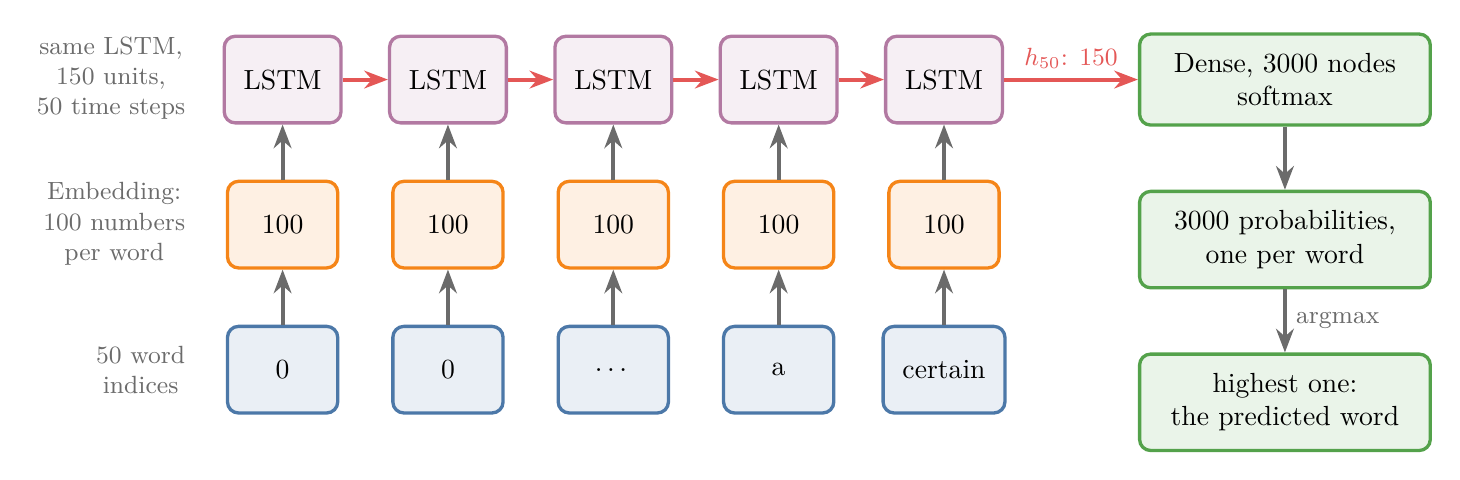
\begin{tikzpicture}[node distance=0.9cm]
  % input words
  \foreach \k/\w in {1/0, 2/0, 3/{\dots}, 4/a, 5/certain} \node[box=cblue, minimum width=1.4cm] (x\k) at (2.1*\k, 0) {\w};
  \node[note, anchor=east] at (1.0, 0) {50 word\\indices};
  % embedding vectors
  \foreach \k in {1,...,5} \node[box=corange, minimum width=1.4cm, above=0.7cm of x\k] (e\k) {100};
  \node[note, anchor=east] at (1.0, 1.85) {Embedding:\\100 numbers\\per word};
  \foreach \k in {1,...,5} \draw[arrow] (x\k) -- (e\k);
  % LSTM cells
  \foreach \k in {1,...,5} \node[box=cpurple, minimum width=1.4cm, above=0.7cm of e\k] (l\k) {LSTM};
  \node[note, anchor=east] at (1.0, 3.7) {same LSTM,\\150 units,\\50 time steps};
  \foreach \k in {1,...,5} \draw[arrow] (e\k) -- (l\k);
  \foreach \k [evaluate=\k as \n using int(\k+1)] in {1,...,4} \draw[arrow, draw=cred] (l\k) -- (l\n);
  % output
  \node[box=cgreen, right=1.7cm of l5, text width=3.2cm] (d) {Dense, 3000 nodes\\softmax};
  \draw[arrow, draw=cred] (l5) -- node[above, note, text=cred] {$h_{50}$: 150} (d);
  \node[box=cgreen, below=0.8cm of d, text width=3.2cm] (p) {3000 probabilities,\\one per word};
  \draw[arrow] (d) -- (p);
  \node[box=cgreen, below=0.8cm of p, text width=3.2cm] (w) {highest one:\\the predicted word};
  \draw[arrow] (p) -- node[right, note] {argmax} (w);
\end{tikzpicture}
\end{document}
